\section*{Comportamiento}

\begin{enumerate}
  \item Gr\'aficas a gran escala. Se trazan todos los elementos del retardo de extremo a extremo. Para trazar estas gr\'aficas
  usaremos las siguientes l\'ineas en Octave
  \begin{figure}[H]
    \centering
    \begin{lstlisting}[frame=single, breaklines=true, basicstyle=\footnotesize\ttfamily, breakatwhitespace=false, 
      columns=flexible, tabsize=2, showstringspaces=false]

      data = load('output1.txt');
      x = data(:, 1);
      y = data(:, 2);
      plot (x,y, '-o', 'Color', 'k');
      xlabel ('Tiempo de sesion');
      ylabel ('Retardo de extremo a extremo');
      title ('Grafica a gran escala Traza 1');
      print -dpng "../../Reporte/img/traza1_GE.png";

    \end{lstlisting}
  \end{figure}

  \begin{figure}[h]
      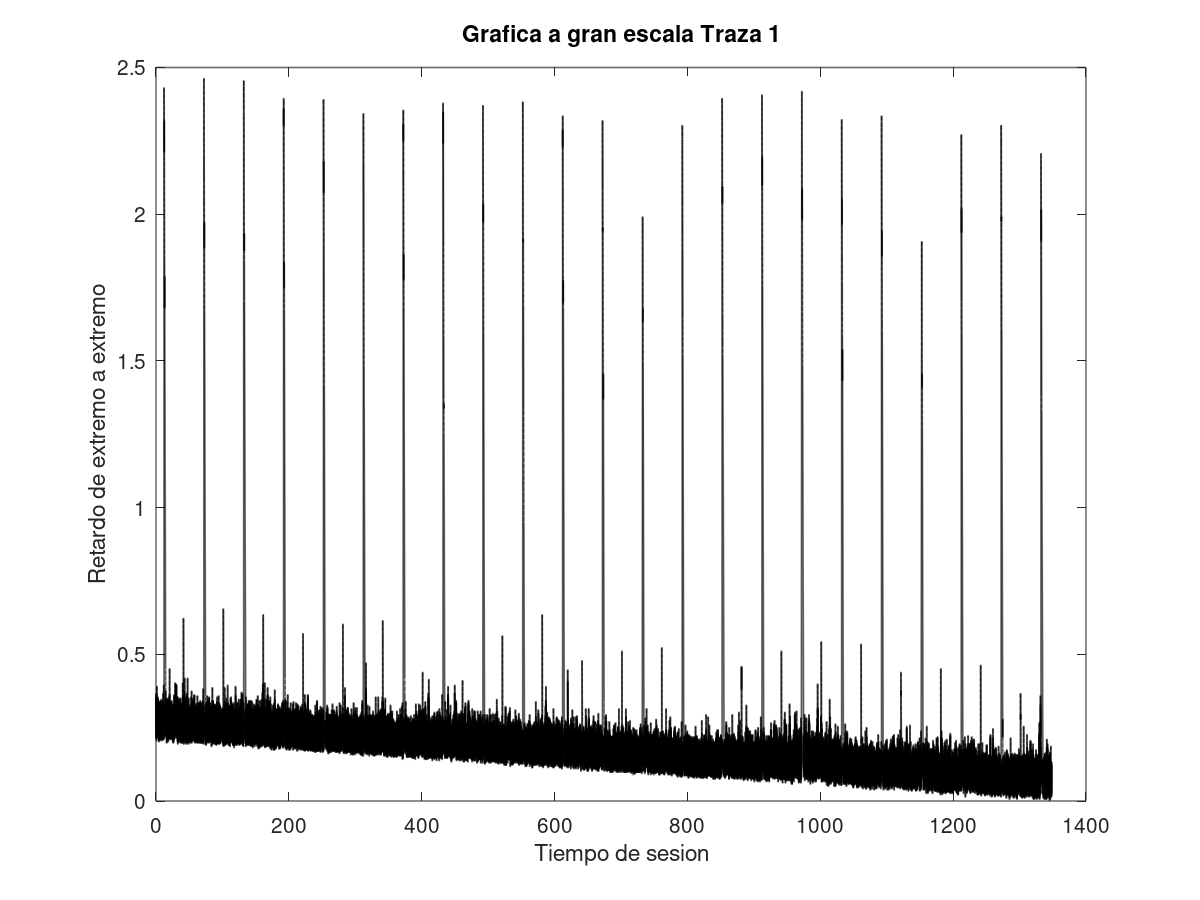
\includegraphics[width=0.45\textwidth]{img/traza1_GE.png}
      \hfill
      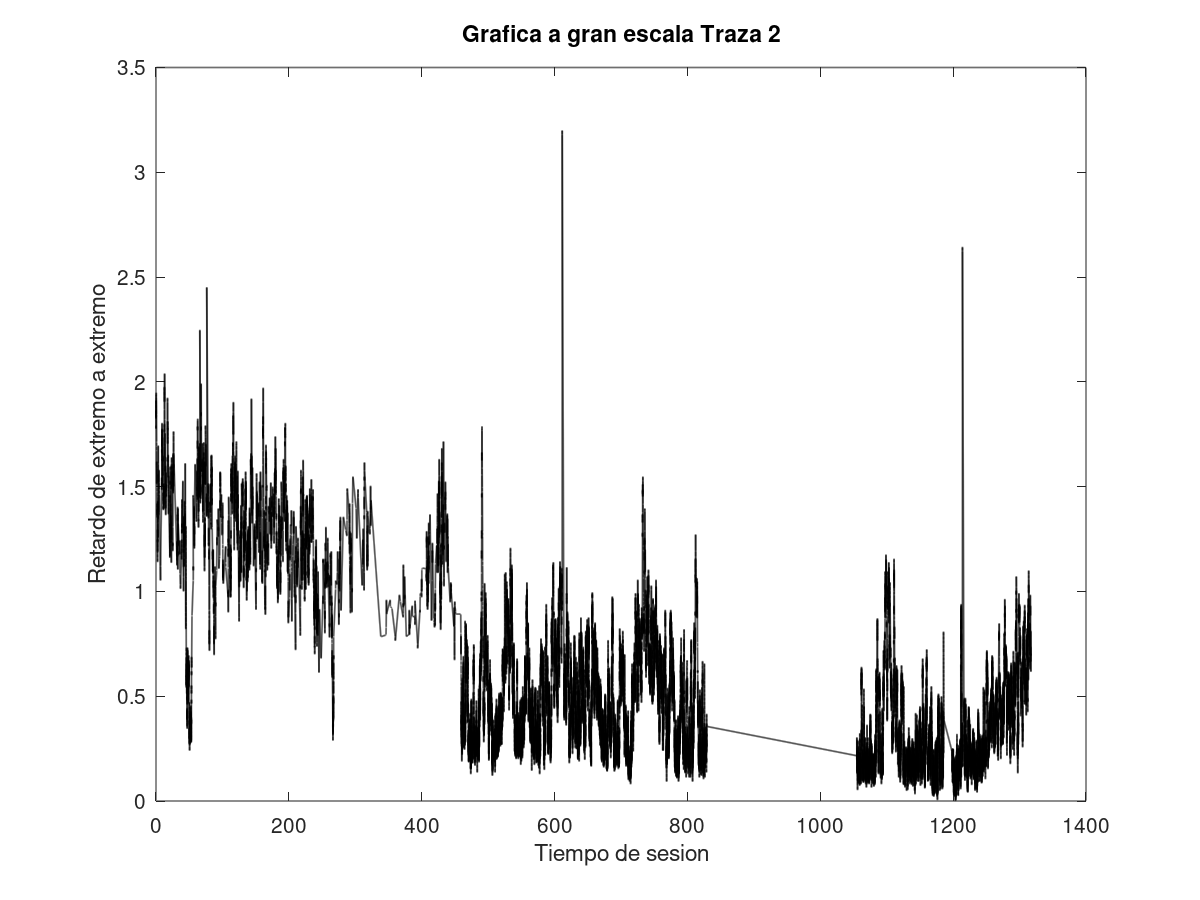
\includegraphics[width=0.45\textwidth]{img/traza2_GE.png}
      \vfill
      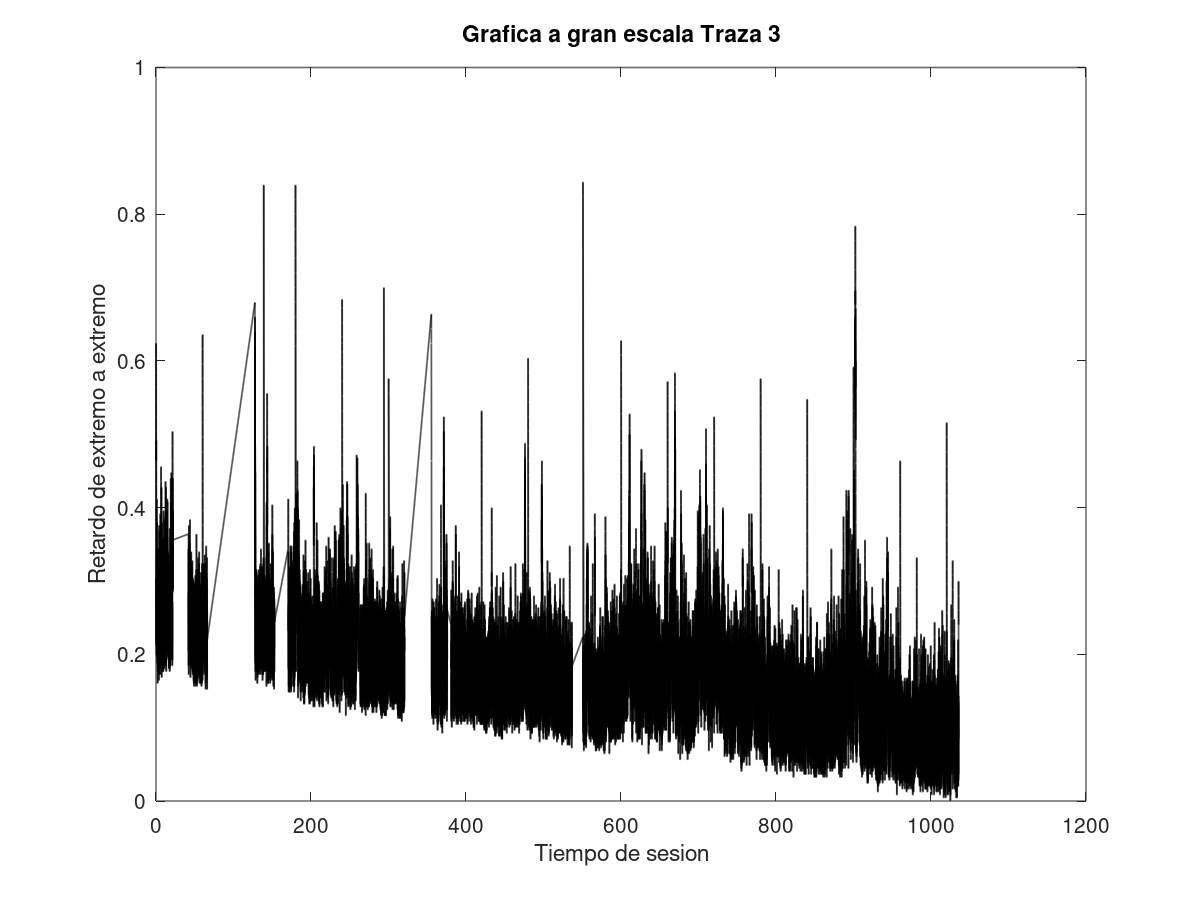
\includegraphics[width=0.45\textwidth]{img/traza3_GE.png}
      \hfill
      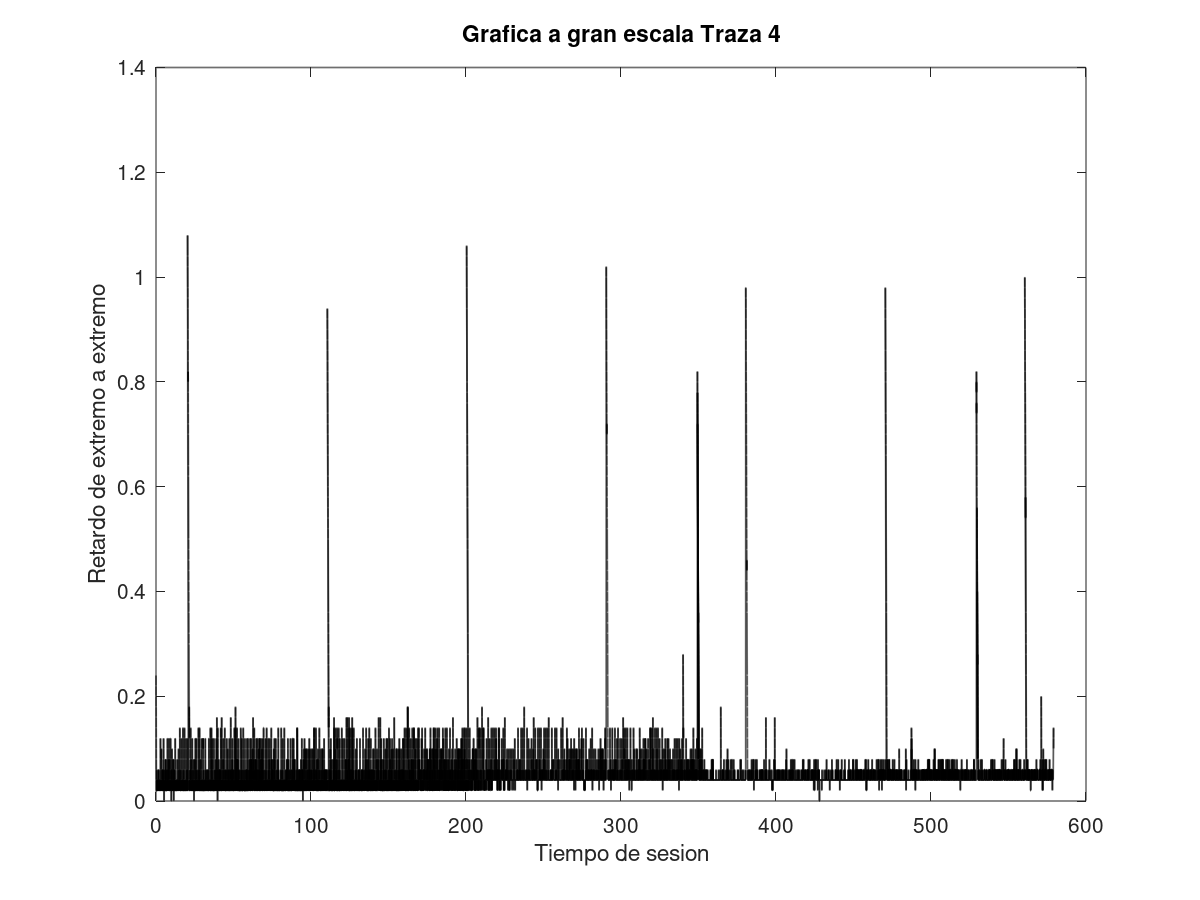
\includegraphics[width=0.45\textwidth]{img/traza4_GE.png}
      \vfill
      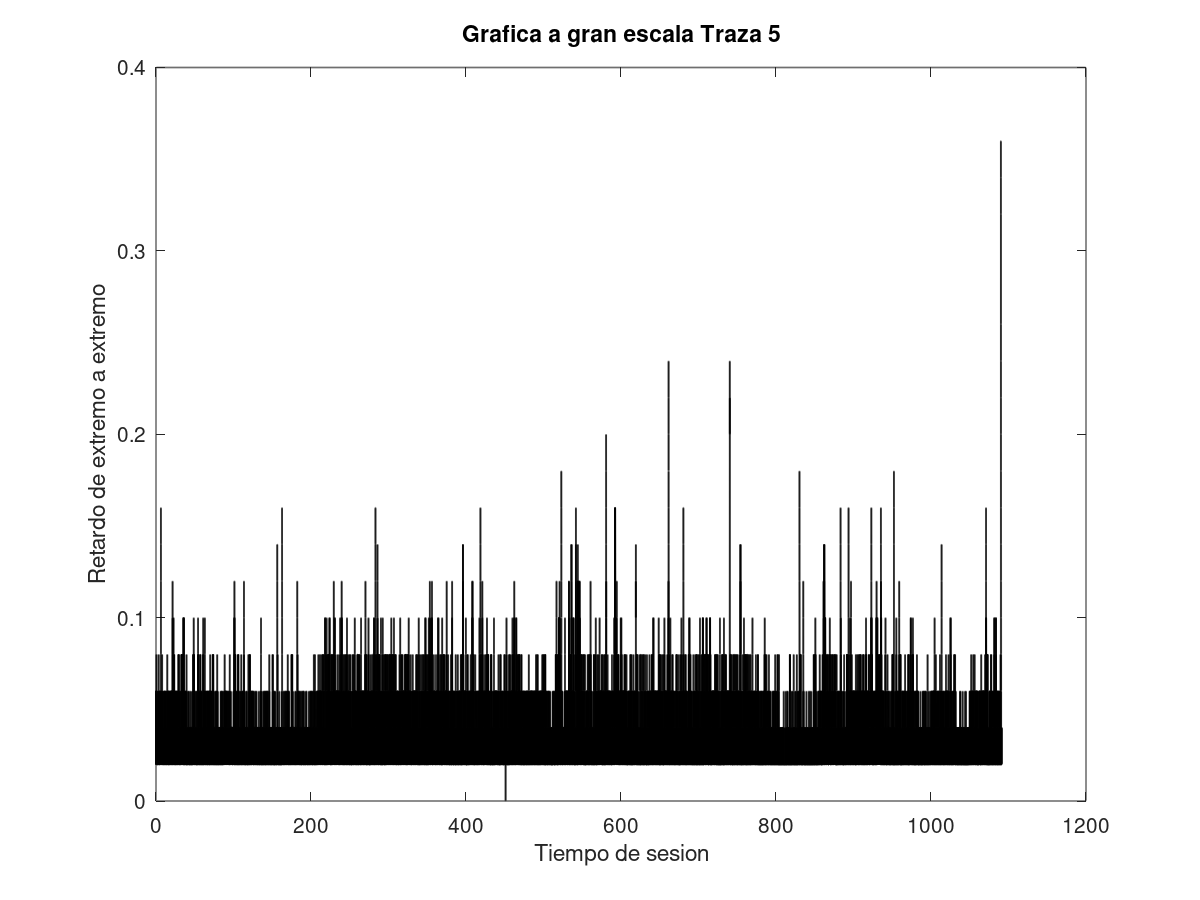
\includegraphics[width=0.45\textwidth]{img/traza5_GE.png}
      \hfill
      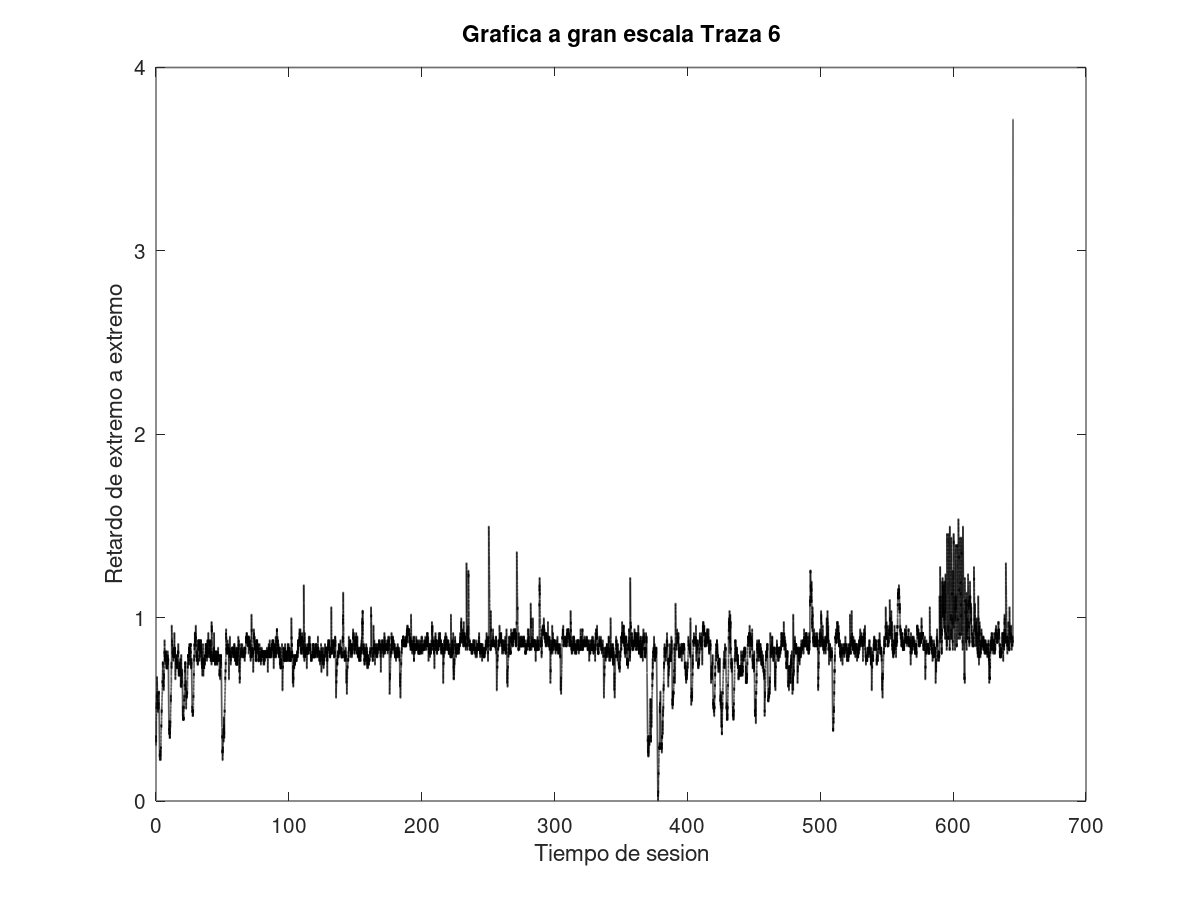
\includegraphics[width=0.45\textwidth]{img/traza6_GE.png}
      \vfill
  \end{figure}


  \item Gr\'aficas a pequeña escala. Se trazan dos o tres frases en la conversaci\'on.
  \noindent El primer paso para poder trazar las gr\'aficas a pequeña escala es acotar las sesiones a unas cuantas frases. Para esto
  usaremos el siguiente script en AWK que solo obtiene los datos de las primeras cuatro frases
  \begin{figure}[H]
    \centering
    \begin{lstlisting}[frame=single, breaklines=true, basicstyle=\footnotesize\ttfamily, breakatwhitespace=false, 
      columns=flexible, tabsize=2, showstringspaces=false, language=AWK]

      # Este script genera un archivo con dos columnas: tiempo de la sesion y retardo extremo a extremo.
      BEGIN{
          #Llama al script que se encarga de obtener la diferencia minima
          temp_file = "output.tmp"
          input_file = ARGV[1]
          command = "awk -f ../Script_3/script3.awk "input_file " > " temp_file
          system(command)
      
          # Procesa la salida del archivo temporal
          while ((getline line < temp_file) > 0) {
              # Procesa cada linea de salida del segundo script
              if (line ~ /Diferencia minima:/) {
                  split(line, fields, ":")
                  tmin = fields[2]
              }
          }
      
          # Limpia el archivo temporal
          system("rm -f " temp_file)
      
          t1_flag = 0
          talkspurts = 1
      }
      
      $1 == "D"{
      
          if (t1_flag == 0){
              t1 = $3
              t1_flag = 1
          }
      
          session_time = ($3 - t1) / 8000
          end_to_end_delay = ($2 - $3 - tmin) / 8000
          print session_time, end_to_end_delay
      }
      
      
      $1 == "!"{
        talkspurts++ # Incrementa el contador al encontrar un espacio de silencio
        if(talkspurts == 11){
          exit # Termina la ejecucion si encuentra cuatro signos "!"
        }
      }
      
    \end{lstlisting}
  \end{figure}

  \noindent El siguiente paso es usar el siguiente script en Octave para poder trazar las gr\'aficas
  \begin{figure}[H]
    \centering
    \begin{lstlisting}[frame=single, breaklines=true, basicstyle=\footnotesize\ttfamily, breakatwhitespace=false, 
      columns=flexible, tabsize=2, showstringspaces=false]

      data = load('output1_PE.txt');
      x = data(:, 1);
      y = data(:, 2);
      stem (x,y, 'Color', 'k');
      xlabel ('Tiempo de sesion');
      ylabel ('Retardo de extremo a extremo');
      title ('Grafica a gran escala Traza 1');
      print -dpng "../../Reporte/img/traza1_PE.png";

    \end{lstlisting}
  \end{figure}

  \begin{figure}[H]
    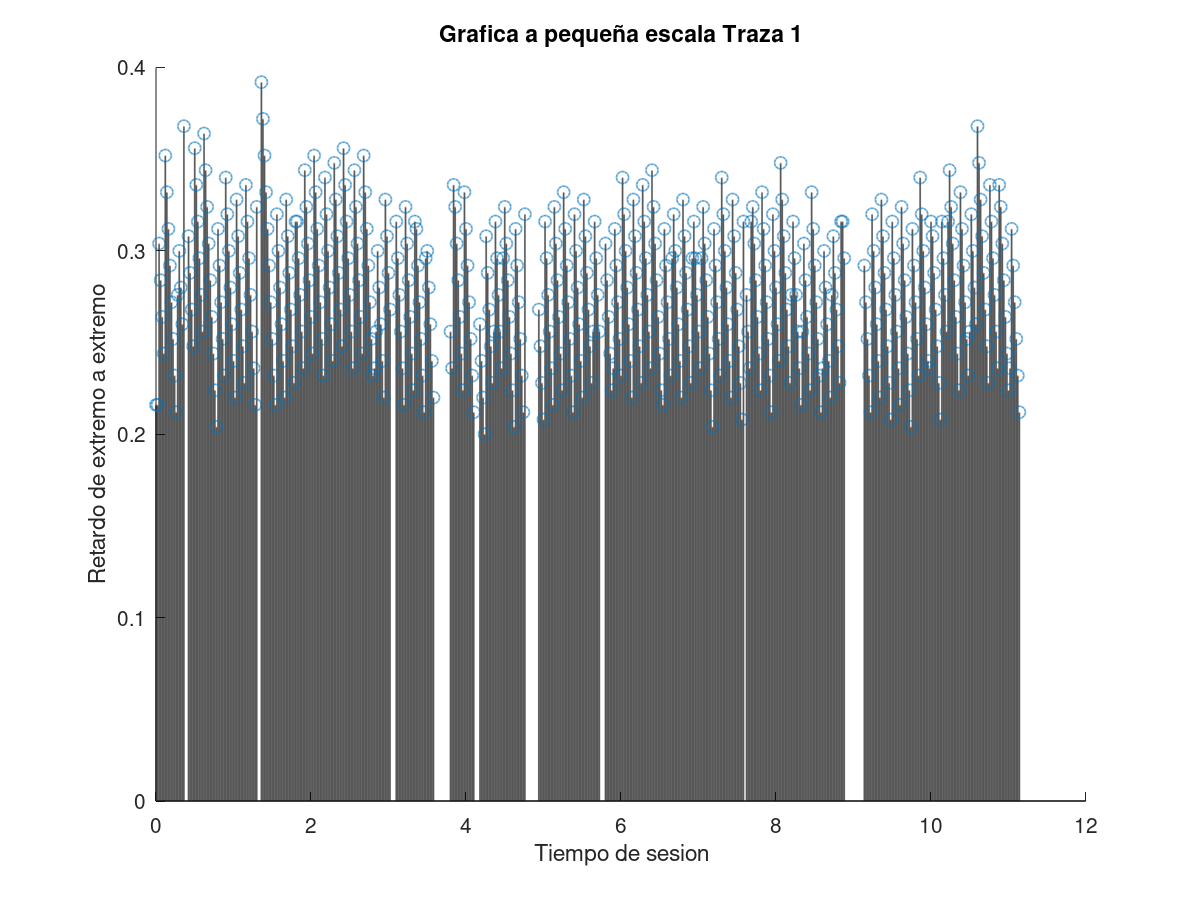
\includegraphics[width=0.45\textwidth]{img/traza1_PE.png}
    \hfill
    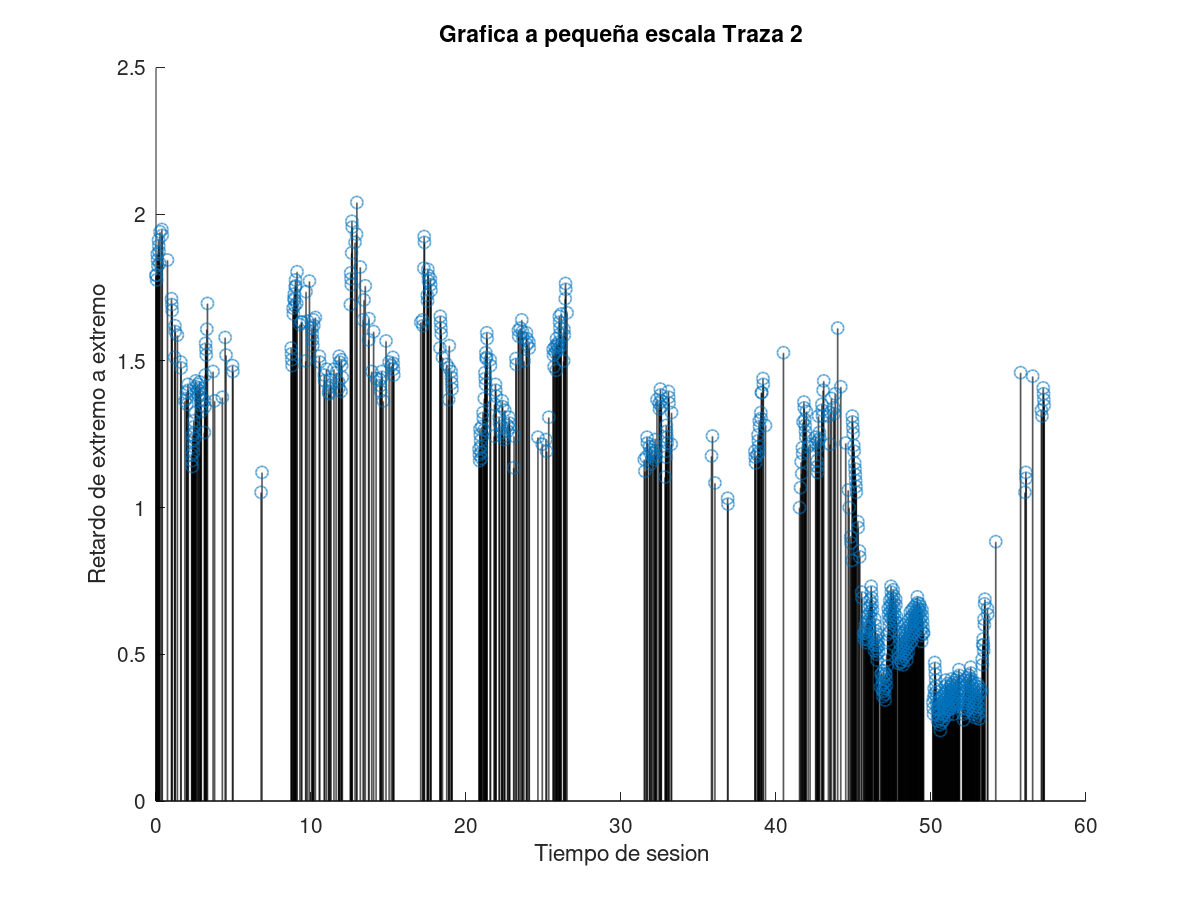
\includegraphics[width=0.45\textwidth]{img/traza2_PE.png}
    \vfill
    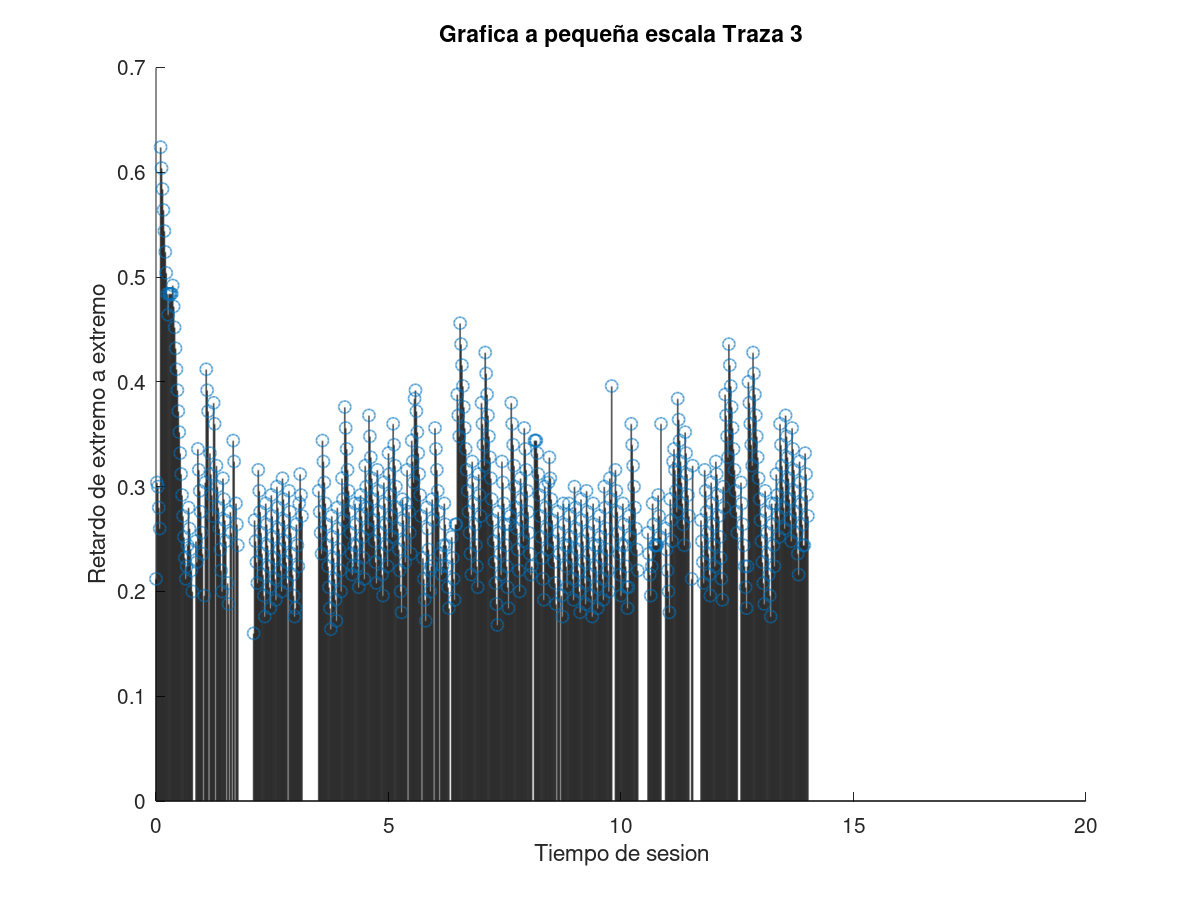
\includegraphics[width=0.45\textwidth]{img/traza3_PE.png}
    \hfill
    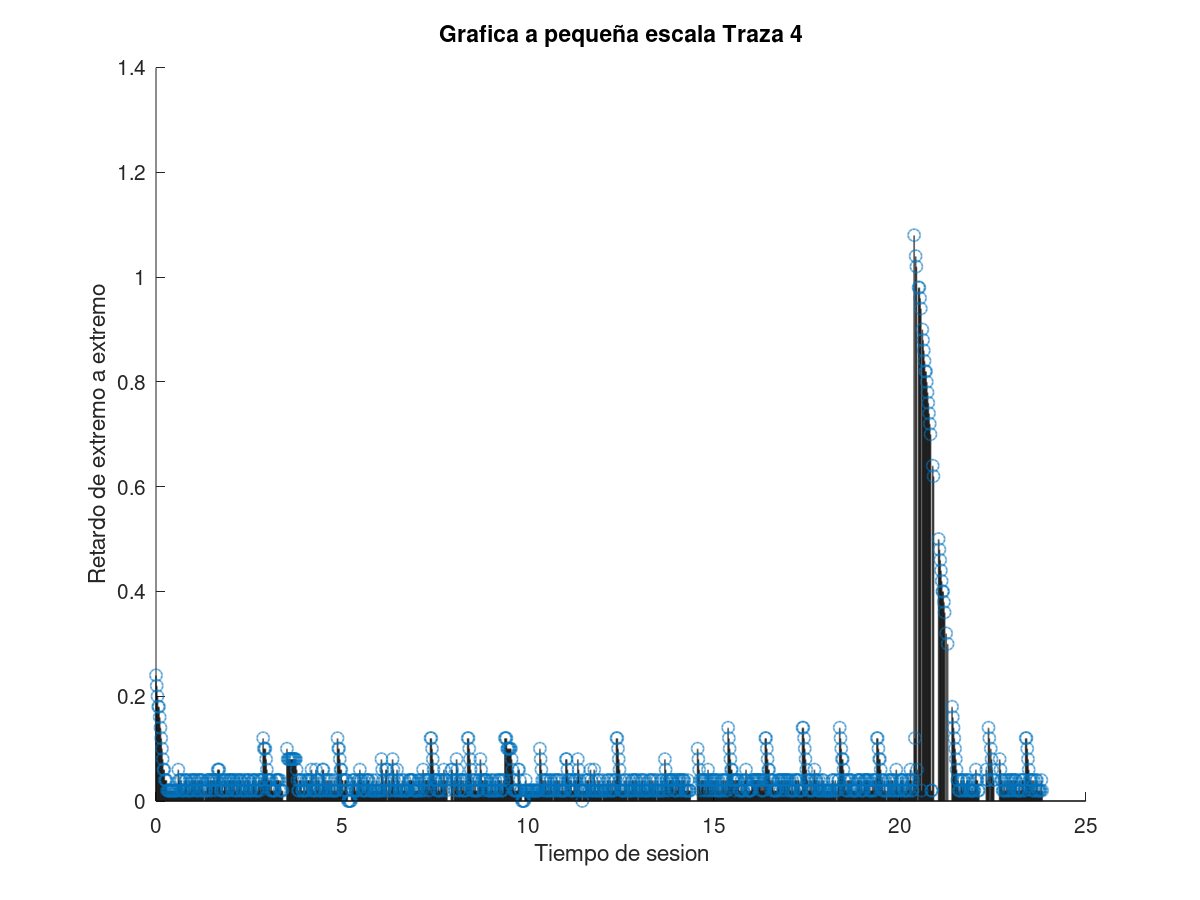
\includegraphics[width=0.45\textwidth]{img/traza4_PE.png}
    \vfill
    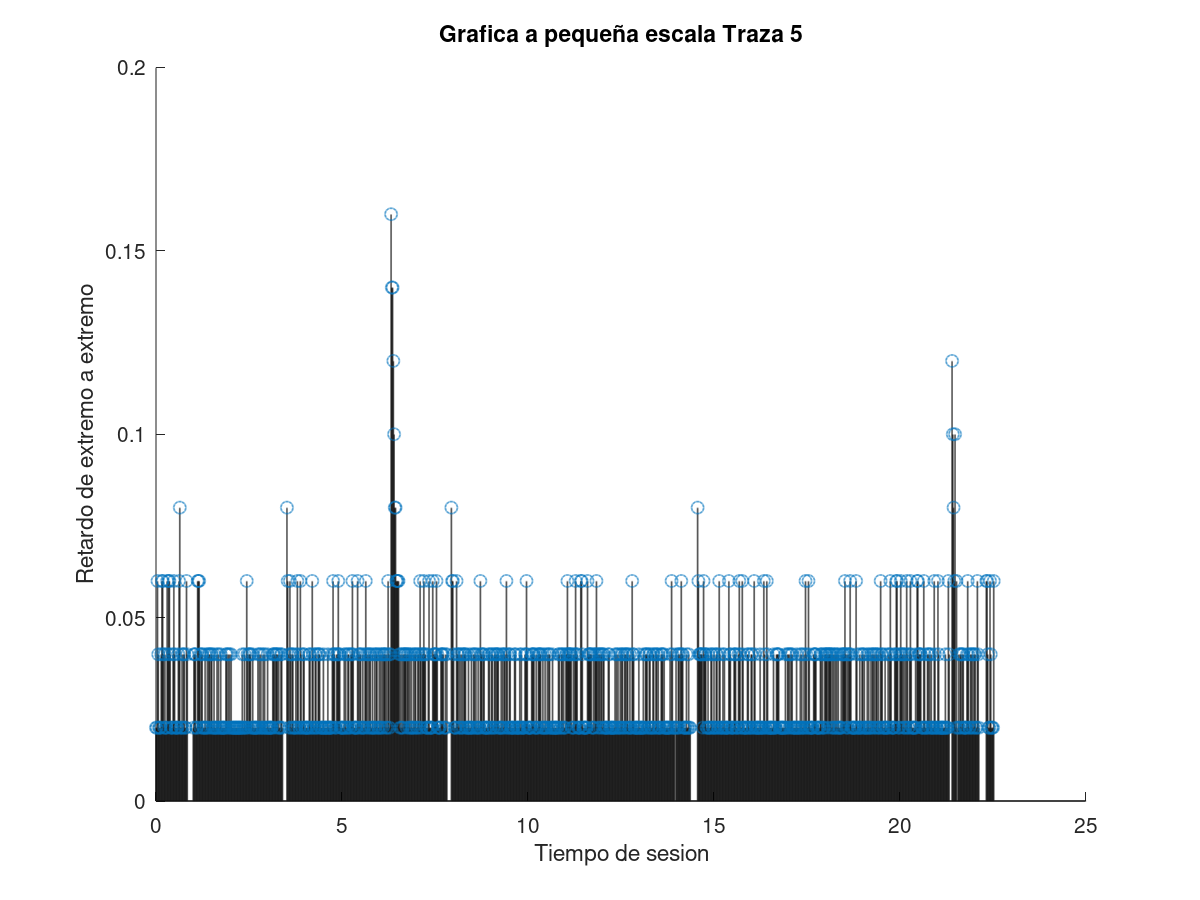
\includegraphics[width=0.45\textwidth]{img/traza5_PE.png}
    \hfill
    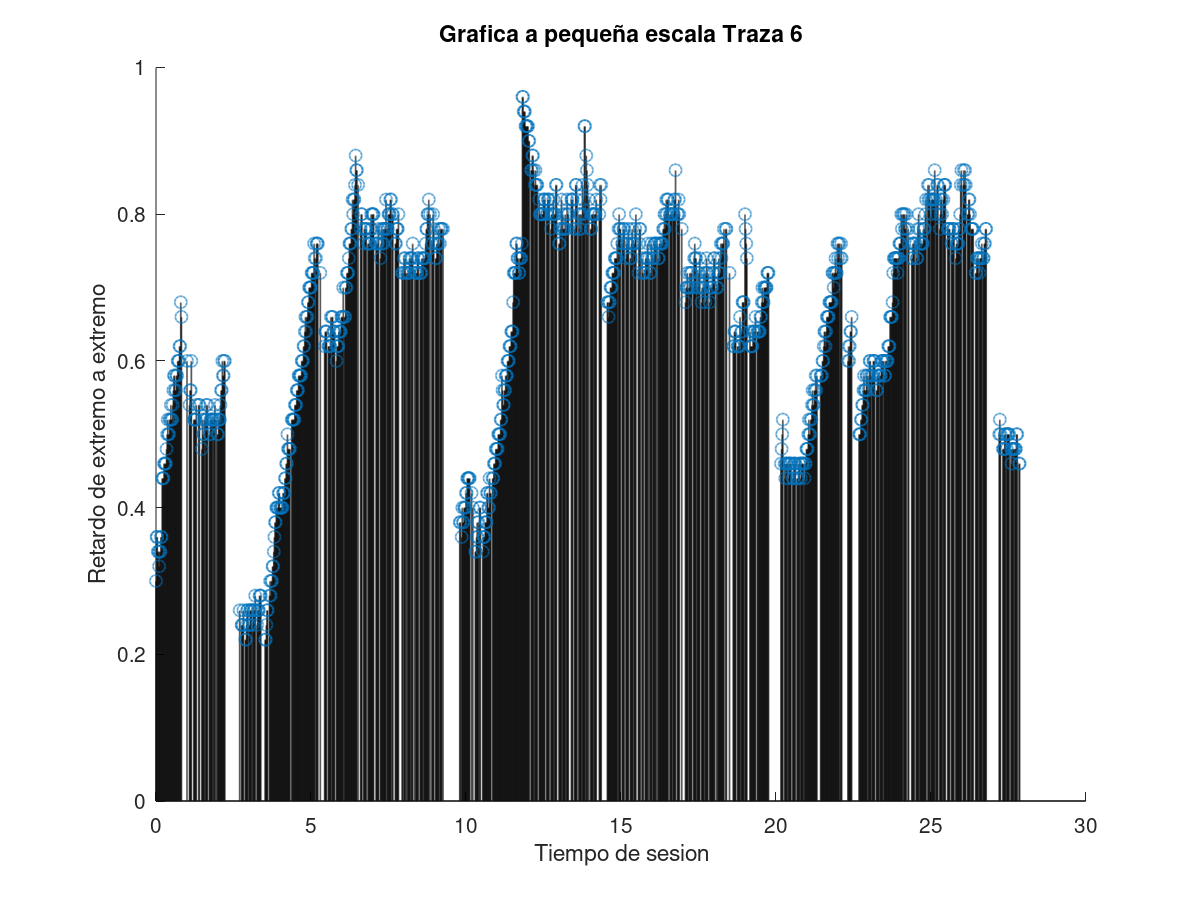
\includegraphics[width=0.45\textwidth]{img/traza6_PE.png}
    \vfill
\end{figure}

\item ¿C\'uales son los fen\'omenos particulares que observa usted en las gr\'aficas que acaba de obtener?
\noindent Se observan tendencias generales en el comportamiento del retardo extremo a extremo, como una pendiente negativa consistente, lo cual
podría indicar una desincronización entre las estampas de tiempo del receptor y el emisor. También se observan se aprecian fluctuaciones grandes
en el retardo extremo a extremo, lo cual podría indicar una congestión en la red. 

\noindent En las gr\'aficas a pequeña escala se observa un an\'alisis m\'as detallado de los eventos individuales, incluyendo las transiciones
entre las frases (\textit{talkspurts}) y los periodos de silencio. Estas gr\'aficas permiten observar el comportamiento más preciso del retardo
entre paquetes conscutivos.

\item Tabla con las estad\'isticas obtenidas
\begin{table}[H]
  \centering
  \begin{tabular}{@{}ccccc@{}}
  \toprule
  \# Traza & \begin{tabular}[c]{@{}c@{}}Total de\\ frases\end{tabular} & \begin{tabular}[c]{@{}c@{}}Total de\\ paquetes\end{tabular} & \begin{tabular}[c]{@{}c@{}}Diferencia\\ mínima\end{tabular} & \begin{tabular}[c]{@{}c@{}}Retardo promedio\\ extremo a extremo\end{tabular} \\ \midrule
  1        & 818                                                       & 56,979                                                      & -641,808                                                    & 0.110536                                                                     \\
  2        & 406                                                       & 24,490                                                      & \multicolumn{1}{l}{-14,643,186}                             & 0.392336                                                                     \\
  3        & 536                                                       & 37,640                                                      & -774,206                                                    & 0.109097                                                                     \\
  4        & 252                                                       & 27,814                                                      & -807,010                                                    & 0.0486863                                                                    \\
  5        & 540                                                       & 52,836                                                      & -944,917                                                    & 0.0224502                                                                    \\
  6        & 299                                                       & 23,293                                                      & -1,489,551                                                  & 0.690046                                                                     \\ \bottomrule
  \end{tabular}
  \end{table}

  \item Empecemos respondiendo a que nos referimos al hablar de \textit{pendiente en el retardo}. Este t\'ermnmino re refiere a una tendencia
  sistem\'atica en los valores del retardo extremo a extremo a lo largo de una sesi\'on. Esta desviaci\'on puede deberse a problemas de sincronizaci\'on
  entre el emisor y el receptor. Los dos métodos que se pueden utilizar para corregir este problema son:
  \begin{description}
    \item[M\'etodo de regresi\'on lineal] - Este m\'etodo ajusta una l\'inea de regresi\'on al conjunto de datos del retardo extremo a extremo y se restan
    los valores ajustados de la pendiente de los valores reales del retardo. Esto permite eliminar cualquier tendencia sistem\'atica en los datos.
    \item[M\'etodo de Ajuste Basado en Referencias Temporales Externas] - Este m\'etodo elimina la dependencia de las estampas de tiempo locales del emisor
    y receptor al sincronizarlas con un reloj externo. Esto permite que los valores del retardo extremo a extremo sean independientes de las estampas de tiempo locales.
  \end{description} 
\end{enumerate}